\documentclass[8pt, a4paper, landscape, includeheadfoot]{extarticle}

% Verwendete Pakete

\usepackage[utf8]{inputenc}
\usepackage[top=0.2cm, 
			bottom=0.0cm, 
			left=1.8 cm, 
			right=0.1 cm, 
			footskip = 2.9pt]{geometry}
\usepackage{babel} % set language to new german
\usepackage{amsmath}
\usepackage{amsfonts}
\usepackage{lmodern}
\usepackage{graphicx}
\setlength{\parindent}{0pt}
\usepackage{ulem} %option rausgenommen
\usepackage[dvipsnames]{xcolor}%option "table" raus
\usepackage{enumitem}
\usepackage{mathabx}
\usepackage{enumitem}
\usepackage{colortbl}
\usepackage{mathtools}
\usepackage{wallpaper}
\usepackage{changepage}
\usepackage{tikz}
\usepackage{tabularx}
\usepackage[skins]{tcolorbox}
\usepackage{lipsum}
\usepackage{multicol}
\usepackage{multirow}
\usepackage{letltxmacro}
\usepackage{tabularx}
\usepackage{float}
\usepackage{amssymb, physics}
\usepackage{empheq}
\usepackage{textcomp} % gensymb dependency
\usepackage{calc} % Multiplikation mit werten ermöglichen
\usepackage[makeroom]{cancel} %Terme durchstreichen
\usepackage{mathtools}
\usepackage{sidecap} %für Bild und Text nebeneinander
%\usepackage{gensymb} % Degree celcius symbol
\usepackage{fancyhdr} % Kopfzeile
\usepackage{romannum} % roman numbers
\usepackage{makecell} % zeilenumbruch in tabellen


% Spalteneinstellungen

\setlength\columnsep{5mm}
\setlength{\columnseprule}{0.5pt}

%FBOX Einstellungen

\setlength{\fboxrule}{0.5pt}

%Kopf und Fusszeile 

\setlength{\headsep}{0.5em}
\setlength{\footskip}{2.9pt}

\pagestyle{fancy}
\fancyhf{}
\lhead{\textbf{\Subject}}
\chead{Page \thepage{}}
\rhead{\CustomAuthor}
\cfoot{}

% Farbe

\def \customColor {RoyalBlue}

% Bullet-Symbol für Aufzählungen
\renewcommand\textbullet{\ensuremath{\bullet}}

% Eingekreiste Nummern für Aufzählungen
\newcommand*\circled[1]{\tikz[baseline=(char.base)]{
		\node[shape=circle,draw,inner sep=1.2pt] (char) {#1};}}

% Schriftart
\renewcommand{\familydefault}{\sfdefault}

%Tabelle Horiz. Grösse
\renewcommand{\arraystretch}{1.5}

%Einheiten
\newcommand{\Einheit}[1]{
	$\bigl[ #1 \bigr]$
}

\newcommand{\EinheitBruch}[2]{
	$\bigl[ \frac{#1}{#2} \bigr]$
}

\newcommand{\Umbruch}{\vfill\null\columnbreak}

% Titel-Block	
\newcommand{\Header}[3]{
	\begin{tcolorbox}  [arc = 0mm,
			colback = \customColor!50!black,
			colframe = \customColor!50!black,
			valign = center,
			fontupper=\color{white}]
		\large \center \textbf{#1} \par
		\huge \textbf{#2} \par
		\vskip 5pt
		\large #3 \par
		\vskip 3pt
		\small Version: \today
	\end{tcolorbox}
}

%Teil-Block
\newcommand{\Abschnitt}[1]{
	\begin{tcolorbox} [arc = 0mm,
			colback = \customColor!50!black,
			colframe = \customColor,
			valign = center,
			before skip = 3mm,
			leftright skip = -0.5mm,
			after skip = 1 mm,
			bottomrule = 0 mm,
			toprule = 0 mm,
			leftrule = 0 mm,
			rightrule = 0 mm,
			fontupper=\color{white}
		]
		\centering\Large\textbf{#1}
	\end{tcolorbox}
}

% Überschrift
\renewcommand{\section}[1]{
	\begin{tcolorbox}[
			arc=0mm,
			colback=\customColor!50!black,
			colframe=white,
			bottomrule = 0 mm,
			toprule = 0 mm,
			leftrule = 0 mm,
			rightrule = 0 mm,
			valign=center,
			left=0.5mm,
			top= 0.7 mm,
			bottom= 0.7 mm,
			fontupper=\color{white},
			before skip = 1mm,
			leftright skip = -0.5mm,
			after skip = 1 mm]

		\textbf{#1}
	\end{tcolorbox}
}

% Abschnitt	
\renewcommand{\subsection}[1]{
	\begin{tcolorbox}[
			arc=0mm,
			colback=\customColor!50,
			colframe=white,
			bottomrule = 0 mm,
			toprule = 0 mm,
			leftrule = 0 mm,
			rightrule = 0 mm,
			valign=center,
			left=0.5mm,
			top=0.2mm,
			bottom=0.2mm,
			before skip = 1mm,
			leftright skip = -0.5mm,
			after skip = 1mm]
		\small \textbf{#1}
	\end{tcolorbox}
}

\renewcommand{\subsubsection}[2]{
	\begin{tcolorbox}[
			arc=0mm,
			colback=gray!50,
			colframe=white,
			bottomrule = 0 mm,
			toprule = 0 mm,
			leftrule = 0 mm,
			rightrule = 0 mm,
			valign=center,
			left=0.5mm,
			top=0.2mm,
			bottom=0.2mm,
			before skip = 1mm,
			leftright skip = -0.5mm,
			after skip = 1mm]
		\small #1 \hfill #2
	\end{tcolorbox}
}

%MATH-BOX, optional commands in {}
\newtcbox{\mathbox}[1][]{%
	nobeforeafter,
	tcbox raise base,
	colframe=blue!30!black,
	colback=blue!20,
	boxrule=1pt,
	arc=1mm,
	before skip = 0mm,
	right = 1mm,
	left=1mm,
	top=0.5mm,
	bottom=0.5mm,
	#1}

\newtcbox{\mathboxnoback}[1][]{%
	nobeforeafter,
	tcbox raise base,
	colframe=black,
	colback=white,
	boxrule=1pt,
	arc=1mm,
	before skip = 0mm,
	right = 1mm,
	left=1mm,
	top=0.5mm,
	bottom=0.5mm,
	#1}

\newcommand{\textbox}[1]{
	\tcbox[
		arc=1mm,
		colback=blue!20,
		colframe=blue!30!black,
		arc=1mm,
		boxrule=1pt,
		right = 1mm,
		left=1mm,
		top=0.5mm,
		bottom=0.5mm,
		before skip = 1mm,
		after skip = 2 mm
	]
	{
		#1
	}
}

\newcommand{\textboxmithead}[2]{
	\begin{tcolorbox}[
			arc=1mm,
			colback=blue!20,
			colframe=blue!30!black,
			arc=1mm,
			boxrule=1pt,
			left=1mm,
			top= 1 mm,
			bottom= 1 mm,
			before skip = 2mm,
			leftright skip = 8mm,
			after skip = 2 mm
		]
		\centering{\textbf{#1}\par}
		#2
	\end{tcolorbox}
}

\newtcolorbox{titlebox}[1][]{
	fonttitle=\bfseries,
	colbacktitle=gray!80,
	enhanced,
	attach boxed title to top center={yshift=-2mm},
	colframe=black,
	colback=white,
	boxrule=1pt,
	arc=1mm,
	before skip = 2mm,
	right = 1mm,
	left=1mm,
	top=0.5mm,
	bottom=0.5mm,
	title=#1}



\def \Subject {CS231a - Computer Vision}
\def \CustomTitle {Cheatsheet}
\def \CustomAuthor {Tim Reinhart - rtim@stanford.edu}

\begin{document}
\pagenumbering{arabic}
\begin{multicols*}{4}
	\Header{\Subject}{\CustomTitle}{\CustomAuthor}

	\section{Matrices}

	\subsection{Matrix Multiplication}

	Matrices can be multiplied with each other in the following manner:

	\begin{center}
		\fbox{
			$A \cdot B = C \hspace{5pt} \Rightarrow \hspace{5pt} c_{ik} = \sum_{j=1}^n a_{ij} \cdot b_{jk}$
		}
	\end{center}

	\begin{center}
		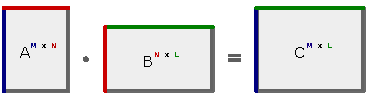
\includegraphics[width = 0.95 \columnwidth]{0_images/Matrixmultiplikation.pdf}
	\end{center}

	\textbf{Associative \& Distributive Laws:}

	\begin{center}
		\parskip3pt
		\begin{align}
			(A\cdot B) \cdot C & = A \cdot (B \cdot C) \nonumber   \\
			(A + B) \cdot C    & = A \cdot C + B \cdot C \nonumber \\
			A \cdot (C + D)    & = A \cdot C + A \cdot D \nonumber
		\end{align}
	\end{center}
	\textbf{Warning!} The commutative law does not apply! Generally, $A\cdot B \neq B \cdot A$.

	\subsection{Transpose}

	The transpose of a matrix is obtained by "mirroring" it along its diagonal.

	\begin{center}
		\textbf{Example:}
		$\begin{pmatrix}
				a & b \\
				c & d \\
				e & f \\
			\end{pmatrix}^T
			=
			\begin{pmatrix}
				a & c & e \\
				b & d & f \\
			\end{pmatrix}$
	\end{center}

	\textbf{Calculation Rules:}

	\vspace{-5mm}
	\begin{minipage}[t]{0.49 \columnwidth}
		\begin{align}
			(A + B)^T     & = A^T + B^T \nonumber     \\
			(A \cdot B)^T & = B^T \cdot A^T \nonumber \\
			(c \cdot A)^T & = c \cdot A^T \nonumber   \\
			(A^T)^T       & = A \nonumber
		\end{align}
	\end{minipage}
	\begin{minipage}[t]{0.49 \columnwidth}
		\begin{align}
			(A^T)^{-1} & = (A^{-1})^T \nonumber \\
			rank(A^T)  & = rank(A) \nonumber    \\
			det(A^T)   & = det(A) \nonumber     \\
			eig(A^T)   & = eig(A) \nonumber
		\end{align}
	\end{minipage}


	\subsection{Inverse}

	The inverse \( A^{-1} \) of \( A \) reverses a multiplication with \( A \). When you multiply \( A \) with \( A^{-1} \), you get the identity matrix.

	\textbf{Properties:}

	\begin{itemize}[leftmargin=0.29cm, itemsep=0pt]
		\item Only square matrices can be invertible.
		\item An invertible matrix is called \textbf{regular}, a non-invertible one \textbf{singular}.
		\item The inverse is unique.
		\item \( A \) is invertible if and only if \( A \) has full rank.
		\item \( A \) is invertible if and only if \( A^T \) is invertible.
		\item \( A \) is symmetric if and only if \( A^{-1} \) is symmetric.
		\item \( A \) is a triangular matrix if and only if \( A^{-1} \) is a triangular matrix.
		\item \( A \) is invertible if and only if \( \text{det}(A) \neq 0 \).
		\item \( A \) is invertible if and only if no eigenvalue \( \lambda = 0 \).
		\item \( A \) and \( B \) are invertible implies \( AB \) is invertible.
	\end{itemize}

	\textbf{Calculation rules:}

	\vspace{-5mm}
	\begin{minipage}[t]{0.49 \columnwidth}
		\begin{align}
			I^{-1}          & = I\nonumber                    \\
			(A^{-1})^{-1}   & = A \nonumber                   \\
			(A^k)^{-1}      & = (A^{-1})^k \nonumber          \\
			(c\cdot A)^{-1} & = c^{-1} \cdot A^{-1} \nonumber \\
			(A\cdot B)^{-1} & = B^{-1} \cdot A^{-1} \nonumber
		\end{align}
	\end{minipage}
	\begin{minipage}[t]{0.49 \columnwidth}
		\begin{align}
			(A^T)^{-1}   & = (A^{-1})^T \nonumber  \\
			rang(A^{-1}) & = rang(A) \nonumber     \\
			det(A^{-1})  & = det(A)^{-1} \nonumber \\
			eig(A^{-1}   & = eig(A)^{-1} \nonumber
		\end{align}
	\end{minipage}

	\subsection{Eigenvalues and Eigenvectors}

	\begin{empheq}[box = \mathboxnoback]{align*}
		\text{Eigenvalues of A: } \det(A - \lambda\cdot I) = 0
	\end{empheq}

	\textbf{Verify Computation}

	\begin{itemize}[leftmargin=0.29cm, itemsep=0.5pt]
		\item Trace(A) = \( a_{11} + a_{22} + \dots + a_{nn} = \sum \lambda_i \)
		\item det(A) = product of \( \lambda_i \)
	\end{itemize}

	\textbf{Eigenvectors: } Kernel of the matrix $A - \lambda_i\cdot I$, where \( \lambda_i \) is the eigenvalue corresponding to the eigenvector.

	\subsection{Determinant}

	\textbf{Block Sentence for Determinant Computation}

	\begin{center}
		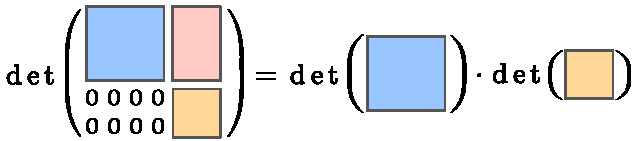
\includegraphics[width = 0.8 \columnwidth]{0_images/Blocksatz.pdf}
	\end{center}

	\subsection{Basic Spaces of a Matrix}

	\textbf{Null Space (Kernel):} Set of all vectors \( v \) such that \( A v = 0 \).\\
	\textbf{Column Space (Range):} Set of all vectors that can be expressed as \( A v \) for some \( v \).\\
	\textbf{Row Space:} Set of all vectors that can be expressed as \( v A \) for some \( v \), equivalent to the column space of \( A^T \).\\

	\Umbruch

	\subsection{Special Matrices}

	\textbf{Identity Matrix \( I \):} Diagonal matrix with ones on the diagonal.\\
	\textbf{Triangular Matrix:} All elements above (upper) or below (lower) the diagonal are zero.\\
	\textbf{Orthogonal Matrix \( Q \):} Satisfies \( Q^T Q = Q Q^T = I \).

	\subsection{QR Decomposition}
	Decomposition of a matrix \( A \) into an orthogonal matrix \( Q \) and an upper triangular matrix \( R \):
	\[
		A = Q \cdot R
	\]

	\subsection{Singular Value Decomposition (SVD)}
	Decomposition of a matrix \( A \) into \( U \), \( \Sigma \), and \( V^T \) where \( U \) and \( V \) are orthogonal, and \( \Sigma \) contains singular values:
	\[
		\mathbf M = \mathbf U \cdot \mathbf \Sigma \cdot \mathbf V^T
	\]

	\begin{itemize}[itemsep=0pt, leftmargin=8pt]
		\item The diagonal entries $\sigma_i = \Sigma_{i i}$ of $ \mathbf \Sigma$ are uniquely determined by $\mathbf M$ and are known as the singular values of $\mathbf M$.
		\item The number of non-zero singular values is equal to the rank of $\mathbf M$.
		\item The columns of ${\displaystyle \mathbf {U} }$ and the columns of ${\displaystyle \mathbf {V} }$ are called left-singular vectors and right-singular vectors respectively.
		\item The columns of $\mathbf U$ and the columns of $\mathbf V$  form two sets of orthonormal bases $\mathbf u_1, \ldots, \mathbf u_m $ and $\mathbf v_1, \ldots, \mathbf v_n$
		\item If they are sorted so that the singular values $\sigma_i$ with value zero are all in the highest-numbered columns (or rows), the singular value decomposition can be written as

		      $$
			      \mathbf{M} = \sum_{i=1}^{r}\sigma_i\mathbf{u}_i\mathbf{v}_i^{*},
		      $$

		      where $r \leq \min\{m,n\}$ is the rank of $\mathbf M$
	\end{itemize}

	\subsubsection{Relation to the Four Fundamental Subspaces}{}

	\begin{itemize}[itemsep=0pt, leftmargin=8pt]
		\item The first \( r \) columns of \( \mathbf{U} \) are a basis of the column space of \( \mathbf{M} \).
		\item The last \( m-r \) columns of \( \mathbf{U} \) are a basis of the null space of \( \mathbf{M}^T \).
		\item The first \( r \) columns of \( \mathbf{V} \) are a basis of the column space of \( \mathbf{M}^T \) (the row space of \( \mathbf{M} \) in the real case).
		\item The last \( n-r \) columns of \( \mathbf{V} \) are a basis of the null space of \( \mathbf{M} \).
	\end{itemize}

	\Umbruch

	\subsubsection{Solving Homogeneous Linear Equations}{}
	\begin{itemize}[itemsep=0pt, leftmargin=8pt]
		\item Equation form: \( \mathbf{A} \mathbf{x} = \mathbf{0} \).
		\item Goal: Find non-zero \( \mathbf{x} \) that satisfies the equation.
		\item \( \mathbf{x} \) is a right null vector of \( \mathbf{A} \).
		\item Characterization: \( \mathbf{x} \) is a right-singular vector for a zero singular value of \( \mathbf{A} \).
		\item If \( \mathbf{A} \) has no zero singular values, there is no non-zero solution. ($\to$ full rank)
		\item Multiple zero singular values allow for solutions that are linear combinations of corresponding right-singular vectors.
		\item Left null vector: \( \mathbf{x}^* \mathbf{A} = \mathbf{0} \) where \( \mathbf{x}^* \) is the conjugate transpose of \( \mathbf{x} \).
	\end{itemize}

	\subsubsection{Total Least Squares Minimization}{}
	\begin{itemize}[itemsep=0pt, leftmargin=8pt]
		\item Objective: Minimize the 2-norm of \( \mathbf{A} \mathbf{x} \) with \( \| \mathbf{x} \| = 1 \).
		\item Solution: Right-singular vector of \( \mathbf{A} \) corresponding to the smallest singular value.
	\end{itemize}

	\subsubsection{Range, Null Space, and Rank}{}
	\begin{itemize}[itemsep=0pt, leftmargin=8pt]
		\item SVD gives explicit representation of matrix's range and null space.
		\item Null space: Spanned by right-singular vectors for zero singular values of \( \mathbf{M} \).
		\item Range: Spanned by left-singular vectors for non-zero singular values of \( \mathbf{M} \).
		\item Rank: Number of non-zero singular values, matching non-zero diagonal elements in \( \mathbf{\Sigma} \).
		\item Effective rank: Determined by singular values, considering numerical errors that might lead to small non-zero singular values.
	\end{itemize}

	\subsubsection{Low-Rank Matrix Approximation}{}
	\begin{itemize}[itemsep=0pt, leftmargin=8pt]
		\item Problem: Approximate \( \mathbf{M} \) with \( \tilde{\mathbf{M}} \) of specific rank \( r \), minimizing the Frobenius norm of their difference.
		\item Solution via SVD:
		      \[
			      \tilde{\mathbf{M}} = \mathbf{U} \tilde{\mathbf{\Sigma}} \mathbf{V}^*,
		      \]
		      where \( \tilde{\mathbf{\Sigma}} \) has only the \( r \) largest singular values, others set to zero.
	\end{itemize}

	\subsection{Homogeneous Coordinates}
	\begin{itemize}[itemsep=0pt, leftmargin=8pt]
		\item Definition: Extends traditional coordinates by adding an extra dimension.
		\item Example: Point \( (x, y) \) in Cartesian coordinates becomes \( (wx, wy, w) \) in homogeneous coordinates, where \( w \neq 0 \).
		\item Applications: Used in computer graphics and computer vision for handling affine and perspective transformations.
		\item Conversion: From homogeneous to Cartesian coordinates by dividing each component by the last coordinate (if non-zero).
		\item \textbf{Point at infinity: } $x_\infty = \begin{bmatrix}
				      x \\ y\\ 0
			      \end{bmatrix}$
	\end{itemize}

	\subsection{Types of Geometric Transformations}
	This section outlines four major types of geometric transformations, each preserving different properties of shapes and spaces. Each type includes an example of how a point in homogeneous coordinates is transformed.

	\subsubsection{Isometric Transformations}{}
	\begin{itemize}[itemsep=0pt, leftmargin=8pt]
		\item Property Preserved: Distances between points.
		\item Also known as rigid transformations, include rotations, translations, and reflections.
		\item Example:
		      $$
			      p' = \begin{bmatrix} \cos \theta & -\sin \theta & t_x \\ \sin \theta & \cos \theta & t_y \\ 0 & 0 & 1 \end{bmatrix} \begin{bmatrix} x \\ y \\ 1 \end{bmatrix}
		      $$
		      for rotation by \( \theta \) and translation by \( (t_x, t_y) \).
	\end{itemize}

	\subsubsection{Similarity Transformations}{}
	\begin{itemize}[itemsep=0pt, leftmargin=8pt]
		\item Property Preserved: Shape of figures $\to$ ratio of lengths and angles
		\item Encompasses isometric transformations along with scaling; angles and relative proportions are maintained.
		\item Example:
		      $$
			      \begin{bmatrix}
				      s \cos \theta & -s \sin \theta & t_x \\
				      s \sin \theta & s \cos \theta  & t_y \\
				      0             & 0              & 1
			      \end{bmatrix}
			      \begin{bmatrix}
				      x \\ y \\ 1
			      \end{bmatrix} =
			      \begin{bmatrix}
				      SR & t \\
				      0  & 1
			      \end{bmatrix}
			      \begin{bmatrix}
				      x \\ y \\ 1
			      \end{bmatrix}
		      $$
		      where \( s \) is the scale factor, $S = \begin{bmatrix}
				      s & 0 \\
				      0 & s
			      \end{bmatrix}$ and  \( \theta \) the rotation angle.
	\end{itemize}

	\Umbruch

	\subsubsection{Affine Transformations}{}
	\begin{itemize}[itemsep=0pt, leftmargin=8pt]
		\item Property Preserved: Points, straight lines, parallelism of lines.
		\item Includes translations, scaling, rotations, and shearing; more general than similarity transformations.
		\item Maps \textbf{points at infinity} to points at infinity!
		\item Example:
		      $$p' = \begin{bmatrix} a & b & t_x \\ c & d & t_y \\ 0 & 0 & 1 \end{bmatrix} \begin{bmatrix} x \\ y \\ 1 \end{bmatrix} $$
		      where matrix elements \( a, b, c, \) and \( d \) define the linear transformation.
	\end{itemize}

	\subsubsection{Projective Transformations / Homographies}{}
	\begin{itemize}[itemsep=0pt, leftmargin=8pt]
		\item Property Preserved: Collinearity of points (lines are preserved).
		\item Can map parallel lines to a converging point, typically used in perspective projections.
		\item Generally maps \textbf{points at infinity} to points no longer at infinity!
		\item Example:
		      $$
			      p' = \begin{bmatrix} a & b & t_x \\ c & d & t_y \\ e & f & g \end{bmatrix} \begin{bmatrix} x \\ y \\ 1 \end{bmatrix}
		      $$
		      where the elements \( e, f, \) and \( g \) introduce the projective distortion.
	\end{itemize}

	\section{Geometry}
	\subsection{2D Lines with homogeneous coordinates}

	Given $ x = [x \, y \, 1]^T$ and $l = [a  \, b  \, c]^T$, then the line eqation is given by:
	$$
		l^T x = 0
	$$
	Slope: $-\frac{a}{b}$, y-intercept: $-\frac{c}{b}$
	\paragraph{Finding $l$}
	Given points $x_1$ and $x_2$, we find $l$ by:
	$$
		\begin{bmatrix}
			a \\ b \\ c
		\end{bmatrix} = \begin{bmatrix}
			x_1 \\ y_1 \\ 1
		\end{bmatrix} \times \begin{bmatrix}
			x_2 \\ y_2 \\ 1
		\end{bmatrix}
	$$
	\paragraph{Finding intersection}
	Given $l_1$ and $l_2$, we find $x$ by:
	$$
		\begin{bmatrix}
			wx \\ xy \\ w
		\end{bmatrix} = \begin{bmatrix}
			a_1 \\ b_1 \\ c_1
		\end{bmatrix} \times \begin{bmatrix}
			a_2 \\ b_2 \\ c_2
		\end{bmatrix}
	$$
	\paragraph{Parallel Lines}For parallel lines $l$ and $l'$, we have the same slope, i.e. $\frac{a}{b} = \frac{a'}{b'}$. Their intersection is given by:
	$$
		l \times l' \propto \begin{bmatrix}
			b \\ -a \\ 0
		\end{bmatrix} = x_\infty
	$$
	All parallel lines (same slope) pass through the same point at infinity (\textbf{ideal point}).


	\section{Camera Matrix Model}
	Parameters:
	\begin{itemize}[itemsep=0pt, leftmargin=8pt]
		\item Focal length $f$
		\item Translation $c_x, c_y$: Image plane and digital image coordinates can differ by a translation
		\item Change of units: $k$ and $l$ change the units from $cm$ to pixels for each axis of the image plane. $\alpha = f\cdot k$ and $\beta = f \cdot l$
	\end{itemize}
	Mapping from 3D point $P$ in camera reference frame to image coordinates $P'$:
	$$
		P' = \begin{bmatrix}
			\alpha \frac{x}{z} + c_x \\
			\beta \frac{y}{z} + c_y
		\end{bmatrix} P
	$$
	Or in homogeneous coordinates:
	\begin{align*}
		P' & = \begin{bmatrix}
			\alpha & 0     & c_x & 0 \\
			0      & \beta & c_y & 0 \\
			0      & 0     & 1   & 0
		\end{bmatrix} \underbracket{\begin{bmatrix}
				x \\ y\\ z \\1
			\end{bmatrix}}_{=P}    \\
		   & = \underbracket{\begin{bmatrix}
				\alpha & 0     & c_x \\
				0      & \beta & c_y \\
				0      & 0     & 1
			\end{bmatrix} }_{=K} \begin{bmatrix}
			I_{3\times 3} & 0
		\end{bmatrix} P
	\end{align*}
	If the world reference frame is different from camera reference frame, we can compute the camera coordinates from world point $P_w$ by:
	$$
		P = \begin{bmatrix}
			R & T \\
			0 & 1
		\end{bmatrix} P_w
	$$
	Where $R$ is the rotation matrix and $T$ is the translation vector (\textbf{extrinsic parameters}).
	Full camera model:
	$$
		P = K\begin{bmatrix}
			R & T
		\end{bmatrix} P_w = MP_w
	$$

	\section{Single View Metrology}
	\subsection{Vanishing Points and Lines}

	Given the direction of a set of parallel 3D lines $d = [a \, b \, c]^T$. The vanishing point $v$ is given by:
	$$
		v = Kd
	$$
	The direction can be computed by:
	$$
		d = \frac{K^{-1}v}{|| K^{-1}v ||}
	$$
	The horizon line $l_{\text{horiz}}$ is the projective transformation of a line at infinity $l_{\infty}$(line that passes through a set of points at infinity). The normal $n$ of a plane in 3D can be computed using
	$$
		n = K^T l_{\text{horiz}}
	$$

	\section{Epipolar Geometry}
	\begin{center}
		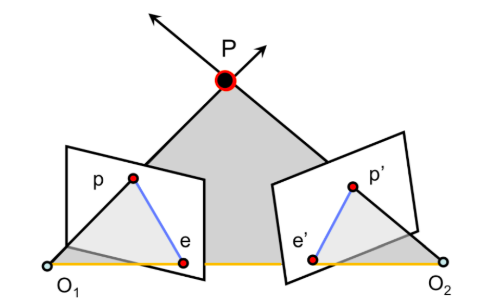
\includegraphics[width=\linewidth]{0_images/epipolar_geometry.png}
	\end{center}
	\begin{itemize}[itemsep=0pt, leftmargin=8pt]
		\item Epipoles: $e, e'$
		\item Epipolar Lines: $\vec{pe},  \vec{p'e'}$
	\end{itemize}
	If you assume that the world reference system is associated with the first camera, then the camera projection matrices are:
	$$
		M = K \begin{bmatrix}
			I_{3\times 3} & 0
		\end{bmatrix}  \quad M' = K' \begin{bmatrix}
			R^T & -R^T T
		\end{bmatrix}
	$$
	\subsection{Essential Matrix}
	Given the rotation $R$ and translation $T$ from the first camera reference frame to the second. The location of $p'$ in the first camera reference frame is:
	$$
		p'_{1} = Rp'_{2} + T
	$$
	The Essential Matrix $E$ is defined for \textbf{canonical cameras}, $K = K' = I$. $E\in\mathbb{R}^{3\times 3}$ has 5 DoF and is defined as:
	$$
		E = \left[T_\times\right] R
	$$
	And the \textbf{epipolar constraint} is
	$$
		p^T E p' = 0
	$$
	Epipolar Lines:
	\begin{itemize}[itemsep=0pt, leftmargin=8pt]
		\item in image plane of camera \textbf{2}: $l' = E^T p$
		\item in image plane of camera \textbf{1}: $l = E p'$
	\end{itemize}
	\paragraph{Dot product with epipoles:} $E^T e = Ee' = 0$

	\subsection{Fundamental Matrix}

	For \textbf{non canonical cameras}. We must define the location of $p$ in the camera reference frame:
	$$
		p_c  = K^{-1}p \quad p'_c = K'^{-1}p'
	$$
	The Fundamental Matrix $F\in\mathbb{R}^{3\times 3}$ has 7 DoF and is defined as:
	$$
		F = K'^{-T}\left[T_\times\right] R K^{-1}
	$$
	Epipolar Lines:
	\begin{itemize}[itemsep=0pt, leftmargin=8pt]
		\item in image plane of camera \textbf{2}: $l' = F^T p$
		\item in image plane of camera \textbf{1}: $l = F p'$
		\item The epipole $e$ lies at the intersection of all epipolar lines $l$.
	\end{itemize}
	Other properties:
	\begin{itemize}[itemsep=0pt, leftmargin=8pt]
		\item $F$ has \textbf{rank $\mathbf 2$}
		\item if $x$ and $x'$ are corresponding image points, then $x'^T F x = 0$
		\item Epipoles: $Fe = 0$ and $F^T e' = 0$
	\end{itemize}

	\subsection{Normalized Eight-Point Algorithm}
	\begin{itemize}[itemsep=0pt, leftmargin=8pt]
		\item $W$ is ill-conditioned for SVD, due to the large image coordinate values in modern cameras. If the image correspondences are all in a small region of the image, then all $p_i$ and $p'_i$ will be very similar, therefore one singular value of $W$ will be very large and the others very small. For SVD to work properly, only one singular value should be near zero.
		\item Solution: Apply a transformation and scaling on the image coordinates.
		\item Origin should be located at the centroid of image points (translation), and the mean squared distance of the transformed image points should be $2$ pixels.
	\end{itemize}
	For \textbf{each camera} we define a transformation $T$. The scaling factor $s$ is given by:
	$$
		s = \sqrt{\frac{2N}{\sum_{i}^{N} || x_i - \bar{x} ||}}
	$$
	where $\bar{x} = \frac{1}{N}\sum_{i}^{N} x_i$. Then the transformation is given by:
	$$
		T = \begin{bmatrix}
			s & 0 & -s \cdot \bar{x}_1 \\
			0 & s & -s \cdot \bar{x}_2 \\
			0 & 0 & 1
		\end{bmatrix}
	$$
	The points are normalized by:
	$$
		q_i = Tp_i \quad q'_i = T'p'_i
	$$
	And the final Fundamental Matrix is given by:
	$$
		F = T'^T F_q T
	$$

	\section{Disparity}

	\begin{center}
		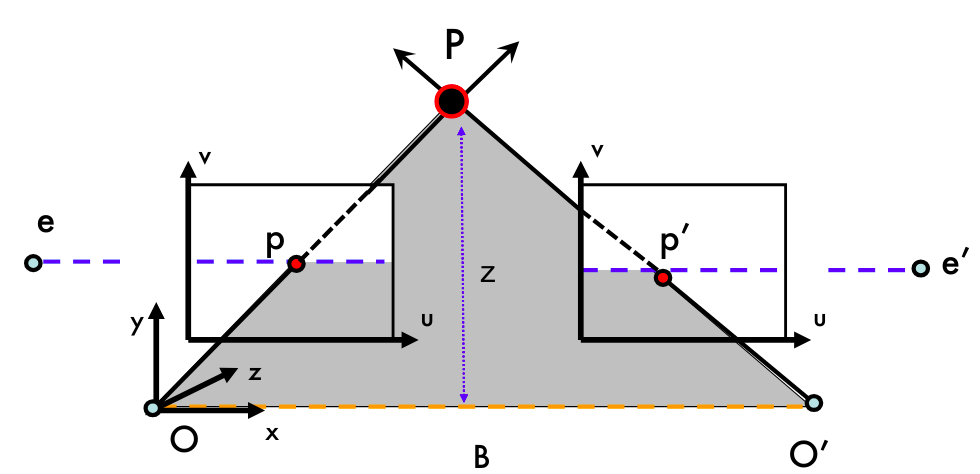
\includegraphics[width=\linewidth]{0_images/disparity.png}
	\end{center}

	$$
		p = \begin{bmatrix}
			p_u \\ p_v \\ 1
		\end{bmatrix} \quad p' = \begin{bmatrix}
			p'_u \\ p'_v \\ 1
		\end{bmatrix}
	$$
	Disparity $d$ is defined as:
	$$
		d = p_u - p'_u \, \propto \,  \frac{B \cdot f}{z}
	$$

	\section{Structure from Motion (SfM)}

	\begin{itemize}[itemsep=0pt, leftmargin=8pt]
		\item $m$ cameras with camera matrix $M_i$
		\item $n$ 3D point measurements $X_j$
		\item location $x_{ij}$ is the projection of $X_j$ in the image plane of camera $i$
	\end{itemize}
	Goal is to recover the $m$ projection matrices $M_i$ (motion) and the $n$ 3D points $X_j$ (structure).

	\Umbruch

	\subsection{Tomasi and Kanade Factorization Method}
	Solves the affine structure from motion problem: Assuming a weak perspective transformation $M$.

	\paragraph{Step 1:} Data Centering. For each image $i$, subtract the centroid $\bar{x}_i$ from image coordinates.

	\paragraph{Step 2: } Build a measurement matrix $D\in\mathbb{R}^{2m \times n}$. Use the SVD of $D = U\Sigma V^T$. We know that $rank(D) = 3$, therefore only three singular values will be nonzero.

	\paragraph{Robust Factorization: } $M = U_3\sqrt{\Sigma_3} \quad S = \sqrt{\Sigma_3}V_3^T$

	Where $M \in \mathbb{R}^{2m \times 3}$ and $S \in \mathbb{R}^{3\times n}$
	$$
		M = \begin{bmatrix}
			A_1 \\ \vdots \\ A_m
		\end{bmatrix} \quad S = \begin{bmatrix}
			X_1 & \hdots & X_n
		\end{bmatrix}
	$$
	Where $A_i$ uses the affine camera model:
	$$
		x = \begin{bmatrix}
			m_1 X \\ m_2X
		\end{bmatrix} = \begin{bmatrix}
			A & b
		\end{bmatrix}X
	$$

	\subsubsection{Ambiguities in Reconstruction}{}
	Any invertible matrix $A\in\mathbb{R}^{3 \times 3}$ may be inserted into the Factorization:
	$$
		D = MS = MAA^{-1}S = (MA)(A^{-1}S) = M'S'
	$$
	Therefore, the solution has \textbf{affine ambiguity}, which means that parallelism is preserved, but the metric scale is unknown.

	\paragraph{Similarity ambiguity:} Occurs when a Reconstruction is correct up to a similarity transform - rotation, translation, scaling. Also known as metric Reconstruction. For calibrated cameras, this is the only ambiguity.

	\subsection{Perspective SfM}
	In the general case, $M$ has 11 DoF, as it is defined up to scale.

	\section{Fitting and Matching}
	\subsection{Least Squares Method}
	\paragraph{Model 1:} $y_i - mx_i -b = 0$
	Error:
	$$
		E = \sum_{i}^{n}\left(y_i - mx_i -b \right)^2
	$$
	Solution:
	$$
		h = \begin{bmatrix}
			m \\b
		\end{bmatrix} = (X^T X)^{-1}X^T Y
	$$
	Where:
	$$
		X = \begin{bmatrix}
			x_1    & 1      \\
			\vdots & \vdots \\
			x_n    & 1
		\end{bmatrix} \quad Y = \begin{bmatrix}
			y_1 \\ \vdots \\ y_n
		\end{bmatrix}
	$$
	Issues: Fails completely for vertical line!

	\paragraph{Model 2:} $ax_i + b y_i + d = 0$

	Distance between points $(x, y, 1)$ and line $(a, b, d)$ is given by $ax + by = d$. Find line to minimize sum of squared perpendicular distances:
	$$
		E = \sum_{i}^{n}\left(ax_i + by_i + d \right)^2
	$$
	Find $h$ s.t. $Ah = 0$. Minimize $||Ah||$ subject to $||h|| = 1$. SVD, $h$ is the last column of $V$.

	Least squares is \textbf{not Robust} to outliers!

	\subsection{RANSAC}
	Robust to outliers and missing data!

	\paragraph{Steps for Eight-Point Algorithm}
	\begin{enumerate}[itemsep=0pt, leftmargin=8pt]
		\item Randomly select the minimum number of points needed to fit a model. Line: 2, 8PA: 8, Homography: 4 correspondences
		\item Fit model to random sample set
		\item Use model to compute the inlier set from the entire dataset
	\end{enumerate}
	Repeat for $M$ iterations, maximize the size of the inlier set

	\section{Volumetric Stereo}

	\subsection{Space Carving}

	\begin{itemize}[itemsep=0pt, leftmargin=8pt]
		\item Requires knowing the camera intrinsics and extrinsics
		\item Produces conservative 3D Reconstructions (no smaller than the actual 3D shape)
		\item Method to find the silhouette of the object in each view is needed
		\item The result is voxels instead of a point cloud, and the degree of accuracy depends on the number of voxels we choose to use.
	\end{itemize}
	\paragraph{Steps}
	\begin{enumerate}[itemsep=0pt, leftmargin=8pt]
		\item Define a working volume, e.g. entire space enclosed by cameras
		\item Divide volume into small units: \textbf{voxels}
		\item Project each voxel into each of the views
		\item If the voxel is not contained by the silhouette in a view, it is discarded.
	\end{enumerate}
	\paragraph{Limitations}
	\begin{itemize}[itemsep=0pt, leftmargin=8pt]
		\item Scales linearly with number of voxel, which increases cubically.
		\item Accuracy depends heavily on the silhouette.
		\item Incapable of modeling certain concavities of an object.
	\end{itemize}

	\subsection{Shadow Carving}
	\begin{itemize}[itemsep=0pt, leftmargin=8pt]
		\item uses self shadows: shadows that an object projects on itself
		\item can estimate concavities better than space carving
		\item produces a conservative volume estimate
	\end{itemize}
	\paragraph{Steps}
	\begin{enumerate}[itemsep=0pt, leftmargin=8pt]
		\item Begins with initial voxel grid
		\item In each view, each light in the array is turned on and off
		\item Identify the shadow in the image plane
		\item find voxels on the surface that are in the visual cone of the Shadow
		\item Use surface voxels allow us to make new visual cone
		\item a voxel that is part of both visual cones cannot be part of the object
	\end{enumerate}
	\paragraph{Limitations}
	\begin{itemize}[itemsep=0pt, leftmargin=8pt]
		\item takes $n + 1$ times longer than space carving ($n$ is nr. of lights)
		\item cannot handle cases where
	\end{itemize}

	\subsection{Voxel coloring}
	\begin{itemize}[itemsep=0pt, leftmargin=8pt]
		\item Uses color consistency instead of contour consistency in space carving
		\item Gives a colored Reconstruction
		\item Object must be Lambertian: the perceived luminance of any part of the objcet does not change with viewpoint location or produces
		\item Voxels need to be processed in a certain order $\to$ cameras cannot be in certain locations
	\end{itemize}
\end{multicols*}

\end{document}
